% -----------------------------------------------------
% CHAPTER 2
% -----------------------------------------------------

\chapter{Week 2 \\ Optimization Algorithms}




% -- Mini-Batch Gradient Descent ------------------------------------------------

\section{Mini-Batch Gradient Descent}

\subsection*{Batch vs. Mini-Batch}

Vectorization allows you to efficiently compute on m examples.
\[ \underset{(n_X, m)}{X} = [x_1, \ldots, x_m] \]
\[ \underset{(1, m)}{Y} = [y_1, \ldots, y_m] \]

What if $m=5,000,000$?

We create batches:
\[ X^{\{1\}}= [x_1,\ldots, x_{1000} ] \]
\[ X^{\{2\}}= [x_{1001},\ldots, x_{2000} ] \]
\[ \vdots \]
\[ X^{\{5000\}}= [x_{4,999,001},\ldots, x_{5,000,000}] \]

and
\[  Y^{\{1\}}= [y_1,\ldots, y_{1000}] \]
\[  Y^{\{2\}}= [y_{1001},\ldots, y_{2000}] \]
\[  \vdots \]
\[  Y^{\{5000\}}= [y_{4,999,001},\ldots, y_{5,000,000}] \]

Now \textit{mini-batch} $t$ will be
\[ (X^{t} , T^{t}) \]

\newpage

\subsection*{Mini-Batch Gradient Descent}

Running one epoch (single pass over the whole training set):

\begin{algorithm}
    \caption*{Mini-Batch Gradient Descent}
    \begin{algorithmic}[1]
    \For{$t = 1$ to $5000$}

        \BlockComment{Forward propagation on $X^{\{t\}}$}
        \State $Z^{[1]} = W^{[1]}X^{\{t\}} + b^{[1]}$
        \State $A^{[1]} = g^{[1]}(Z^{[1]})$
        \State $\ldots$
        \State $Z^{[L]} = W^{[L]}A^{[L-1]} + b^{[L]}$
        \State $A^{[L]} = g^{[L]}(Z^{[L]})$
        
        \BlockComment{Compute cost on $Y^{\{t\}}$}
        \State $\mathcal{J}^{\{t\}} = \frac{1}{m} \sum_{i=1}^{m} \mathcal{L}(\hat{y}^{(i)}, y^{(i)}) + \frac{\lambda}{2m} \sum_{l=1}^{L} ||W^{[l]}||_F^2$ 

        \BlockComment{Backward propagation on $\mathcal{J}^{\{t\}}$}
        \State $dW = \ldots$    
        \State $db = \ldots$
        
        \BlockComment{Update parameters}
        \State $W^{[l]} = W^{[l]} - \alpha dW^{[l]}$
        \State $b^{[l]} = b^{[l]} - \alpha db^{[l]}$
    \EndFor
    \end{algorithmic}
\end{algorithm}

\newpage

\subsection*{Understanding and Training with Mini-batch Gradient Descent}

When training on a whole data set, the cost should decrease with each iteration.

When training on mini-batches, in each iteration we calculate $\mathcal{J}^t$  using $X^t$  and $Y^t$, so on each iteration we calculate the cost on a different data set. Hence we can expect the cost to trend downwards, but not to decrease on every iteration.

\begin{figure}[htbp]
    \begin{minipage}[t]{\textwidth}
        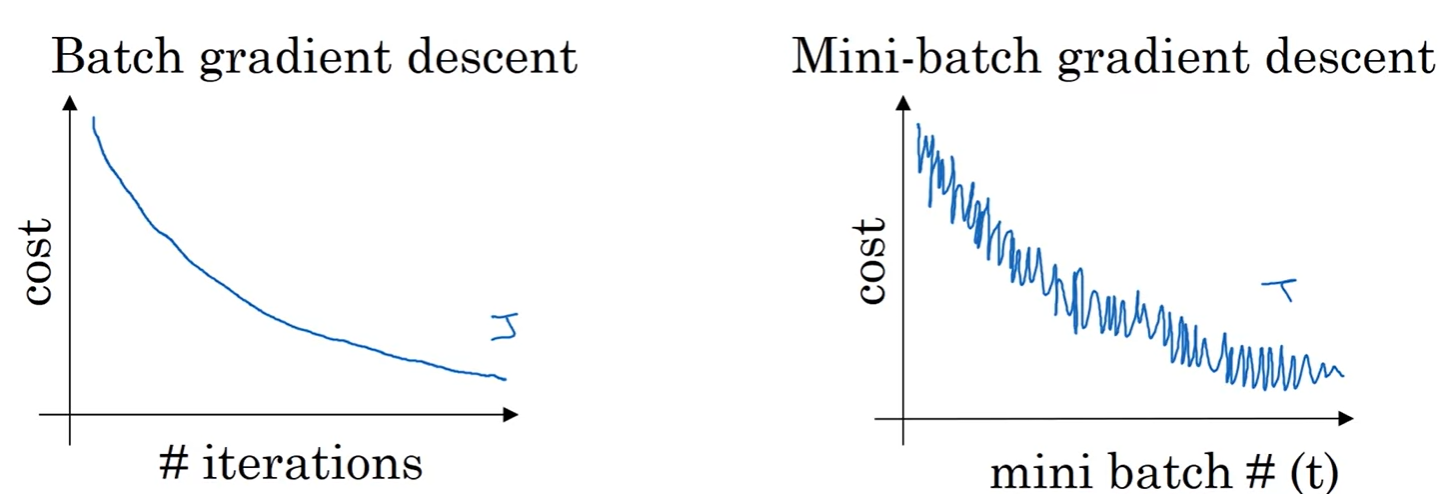
\includegraphics[width=\linewidth]{images/batch_vs_minibatch_gd.png}
    \end{minipage}
\end{figure}

\subsubsection*{Choosing the Mini-Batch Size}

If $m_{batch}=m$, then we have batch gradient descent and $(X^{\{t\}}, Y^{\{t\}} )=(X, Y)$. This is impractical for large data sets. \\
If $m_{batch}=1$, then we have stochastic gradient descent and $(X^{\{t\}}, Y^{\{t\}} )=(x^{(t)},y^{(t)} )$. This takes a long time to converge.

\begin{figure}[htbp]
    \begin{minipage}[t]{\textwidth}
        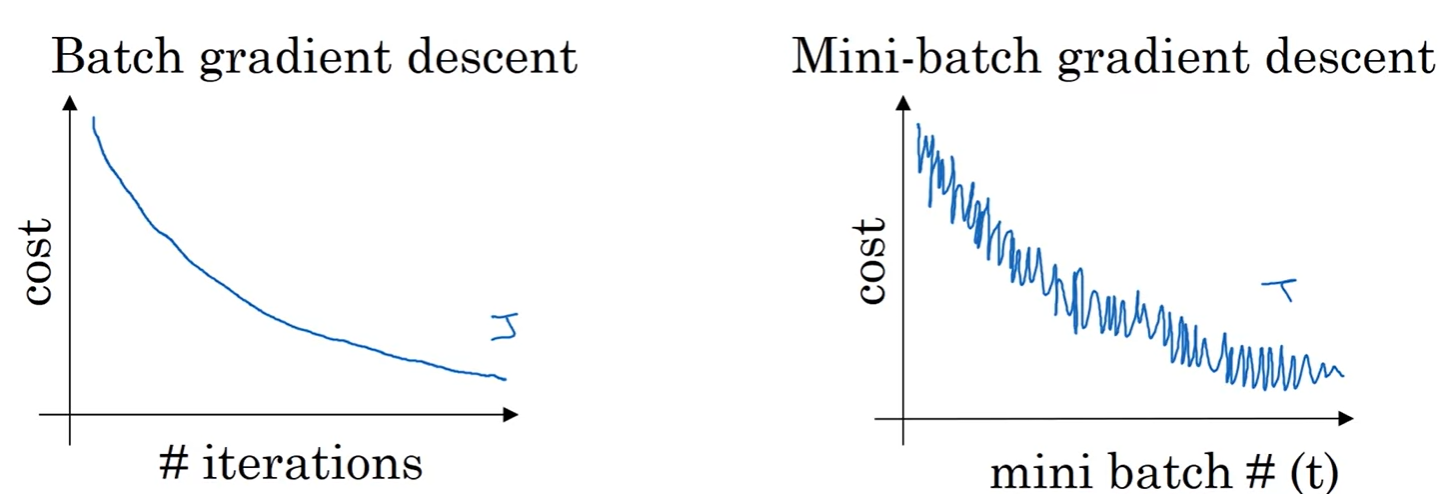
\includegraphics[width=\linewidth]{images/batch_vs_minibatch_gd.png}
        \end{minipage}
\end{figure}

Batch gradient descent
\begin{itemize}
    \item will converge faster
	\item take a (too) long time per iteration
\end{itemize}
	
Stochastic gradient descent:
\begin{itemize}
    \item will "wander around" more, taking steps in different directions depending on the single example that was used in that step
	\item lose the speedup gained by vectorization
\end{itemize}
	

In practice, for mini-batch gradient descent: $1<m_{batch}<m$
\begin{itemize}
    \item get perf gain from vectorization
	\item make progress without needing to wait for the entire training set to be processed
\end{itemize}

\subsection*{How to choose the batch size?}

If the training set is small $(m<2000)$: Use batch gradient descent.
Otherwise, typical mini-batch sizes are 64, 128, 256, 512 and sometimes (1024).

Make sure that the minibatch fits in memory (CPU or GPU) 





% -- Exponentially Weighted Averages -------------------------------------------

\section{Exponentially Weighted Averages}

Given a series of temperatures

\begin{tabular}{ |l|l| }
    \hline
    $\theta_1$ & 4 \\
    \hline
    $\theta_2$ & 9 \\
    \hline
    $\theta_3$ & 6 \\
    \hline
    $\vdots$ & $\vdots$ \\
    \hline
    $\theta_{180}$ & 15 \\
    \hline
    $\theta_{181}$ & 12 \\
    \hline
    $\vdots$ & $\vdots$ \\
    \hline
\end{tabular}

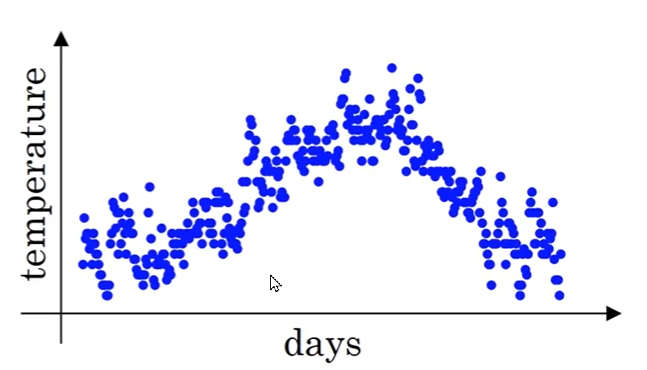
\includegraphics[width=0.7\linewidth]{images/temperatures.png}

Calculate a moving average

\begin{align*}
    V_0 &= 0 \\
    V_1 &= 0.9 V_0 + 0.1 \theta_1 \\
    V_2 &= 0.9 V_1 + 0.1 \theta_2 \\
        & \vdots \\
    V_t &= 0.9 V_{t-1} + 0.1 \theta_t 
\end{align*}

Plotting V in red gives:

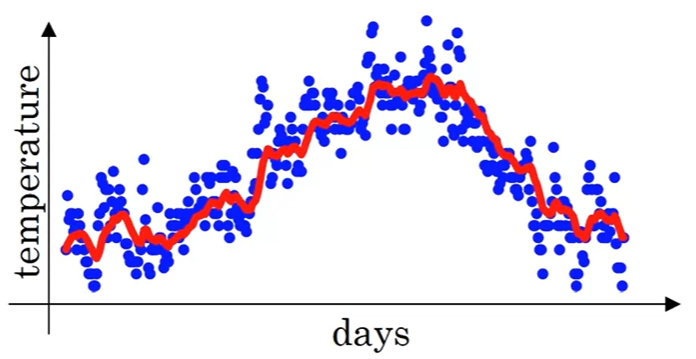
\includegraphics[width=0.7\linewidth]{images/temperatures_one_moving_avg.png}

More generally, we write

\[
    V_t = \beta V_{t-1} + (1 - \beta) \theta_t
\]

We can think of $V_t$  as approximately averaging over  $1/(1-\beta)$  days temperature, 
so for $\beta = 0.9$, we get an average over $1/(1 - 0.9) \approxeq 10$ days.

If we instead use $\beta = 0.98$, we get an average over $1/(1 - 0.98) \approxeq 50$ days, plotted in green below:

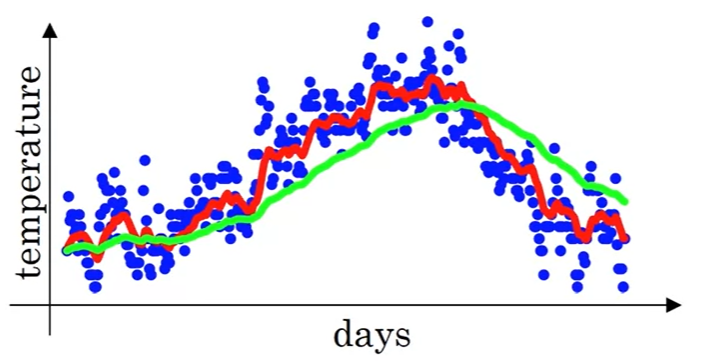
\includegraphics[width=0.7\linewidth]{images/temperatures_two_moving_avgs.png}

The curve is smoother since we are averaging over more values, but have also shifted to the right,
since it ``reacts'' more slowly to changes in temperature (most emphasis is placed on the $V_{t - 1}$ term.)

If we instead use $\beta = 0.5$, we get an average over $ 1 / (1 - 0.5) \approxeq 2$ days, plotted in yellow below:

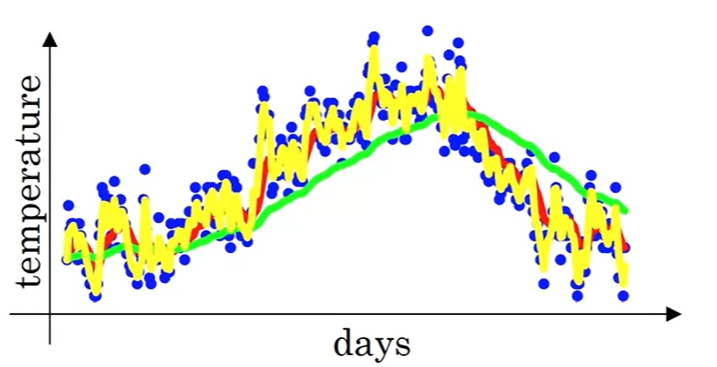
\includegraphics[width=0.7\linewidth]{images/temperatures_three_moving_avgs.png}


\subsection*{Understanding Exponentially Weighted Averages}

\begin{align*}
    V_100 &= 0.9V_{99} + 0.1 \theta_{100} \\
    V_99  &= 0.9V_{98} + 0.1 \theta_{99} \\
    V_98  &= 0.9V_{97} + 0.1 \theta_{98} \\
          & \vdots 
\end{align*}

\begin{align*}
    V_{100} & = 0.1 \theta_{100} + 
                0.9 (0.1 \theta_{99} + 0.9(0.1 \theta_{98} + 0.9(\ldots))) \\
            & = 0.1 (\theta_{100} + 0.9 \theta_{99} +0.9^2 \theta_{98} +0.9^3 \theta_{97} + 0.9^4 \theta_{96} + \ldots) \\
\end{align*}

So the weights of $\theta_n$ are decreasing exponentially.

We have that 
\[
    (1-\epsilon)^{1 / \epsilon} \approxeq 1/e \approxeq 0.35
\]

If we use $1 - \beta$ for $\epsilon$ in the above, we see that when going back $1 / (1 - \beta)$  time points, 
the weight has decreased to $1/e \approxeq 0.35$, which is why we say that we are averaging over that many time points.

\subsection*{Implementing Exponentially Weighted Averages}

Just initialize $V_{\theta}$ to $0$ and keep using it

\begin{align*}
    V_{\theta} &:= 0 \\
    V_{\theta} &:= \beta V_{\theta} + (1 - \beta) \theta_1 \\
    V_{\theta} &:= \beta V_{\theta} + (1 - \beta) \theta_2 \\
    V_{\theta} &:= \beta V_{\theta} + (1 - \beta) \theta_3 \\
    & \ldots 
\end{align*}

\subsection*{Bias Correction in Exponentially Weighted Averages}

For small values of $t$, $V_t$ is biased towards $0$. To overcome this, we introduce a bias factor $1 / (1 - \beta^t )$:
\[
    V_t^{'} = \frac{1}{1 - \beta^t} \cdot V_t = \frac{1}{1 - \beta^t} \cdot (\beta V_{t - 1} + (1 - \beta) \cdot \theta_t)
\]

With $\beta = 0.9, V_0 = 0$:

\begin{align*}
    V_1^{'} &= \frac{1}{1 - 0.9}  \cdot (0.9V_0 + 0.1 \theta_1 ) = \theta_1 \\
    V_2^{'} &= \frac{1}{1 - 0.9^2} \cdot (0.9V_1 + 0.1 \theta_2 )  \\
            &= \frac{1}{1 - 0.9^2} \cdot (0.9 \cdot (0.9V_0 + 0.1 \theta_1 ) + 0.1 \theta_2 )  \\
            &= \frac{1}{0.19} \cdot (0.09 \theta_1 + 0.1 \theta_2 ) = \underline{0.473 \cdot \theta_1 + 0.526 \cdot \theta_2} \\
\end{align*}





% -- Gradient Descent with Momentum --------------------------------------------

\section{Gradient Descent with Momentum}

Use an exponentially weighted average of the gradients to update the weights.

Ordinary gradient descent might "jump around" on its path towards the minimum (blue), 
or even diverge (purple), forcing you to use a small learning rate in order to have it converge.

\includegraphics*[width=0.7\linewidth]{images/gd_without_momentum.png}

We now intruduce momentum, which will dampen the oscillations and allow us to use a larger learning rate.

On iteration t, we compute the gradient $dW, db$ on the current mini-batch, then calculate
\[ V_{dW} =\beta V_{dW} + (1 - \beta) dW \]
\[ V_{db} =\beta V_{db} + (1 - \beta) db \]

We then update the weights:
\[ W \gets W - \alpha V_{dW} \]
\[ b \gets b - \alpha V_{db} \]

This will result in averaging out the gradients, making the algorithm head more directly towards the minimum (in red):

\includegraphics*[width=0.7\linewidth]{images/gd_with_momentum.png}

If we look at gradient descent's path towards the minimum as a ball rolling down the walls of a bowl 
towards the bottom, then in the equations above, e.g.
\[ V_{dW} = \beta V_{dW} + (1 - \beta) dW \]

we can view

\begin{itemize}
	\item the derivative term $dW$ as an acceleration term
	\item the momentum term $V_{dW}$  as the velocity
	\item $\beta$ as a friction factor, preventing unlimited speedup
\end{itemize}
    
In practice, $\beta = 0.9$ seems to work well, and bias correction is rarely used.

A version of momentum sometimes used is
\[ V_{dW} = \beta V_{dW} + dW \]
\[ V_{db} = \beta V_{db} + db \]

where the factor $(1 - \beta)$  has been omitted. The effect is that $V_{dW}$  and $V_{db}$  are scaled 
by a factor $( - \beta)$, and this need to be compensated for in the weight update by setting 
the learning rate $\alpha$ accordingly. A downside of this is that it entangles the hyperparameters $\alpha$ and $\beta$.




% -- RMSprop ------------------------------------------------------------------

\section{RMSprop}

An alternative to Gradient Descent with Momentum is RMSprop (Root Mean Square prop). The idea is to use an exponentially weighted 
average of the squared gradients to update the weights.

On iteration t, we compute the gradient $dW, db$ on the current mini-batch, then calculate

\[ S_{dW} =\beta S_{dW} + (1 - \beta) dW^2 \]
\[ S_{db} =\beta S_{db} + (1 - \beta) db^2 \]

We then update the weights:

\[ W \gets W - \alpha \frac{dW}{\sqrt{S_{dW}}} \]
\[ b \gets b - \alpha \frac{db}{\sqrt{S_{db}}} \]

The S expressions can be seen as exponentially weighted average of the squares of the derivatives.

What we want here is that in the example above, is that $S_{dW}$  will be small, so that in the update of 
$W$ we will divide $dW$ with a small value and take a big step, and that $S_{db}$  will be large,
so that in the update of $b$ we will divide $db$ with a large value and take a small step. 

This will result in a path towards the minimum that is more direct than with ordinary gradient descent.

In practice, to avoid division by $0$, a small term $\epsilon \approx 10^{-8}$  is introduced in the updates:

\[ W \gets W - \alpha \frac{dW}{\sqrt{S_{dW}} + \epsilon} \]
\[ b \gets b - \alpha \frac{db}{\sqrt{S_{db}} + \epsilon} \]




% -- Adam Optimization Algorithm -----------------------------------------------

\section{Adam Optimization Algorithm}

Like momentum and RMSprop, works well across many deep learning architectures.

Adam (Adaptive moment estimation) puts together momentum and RMSrop and combine them in one algorithm:

Set 
\begin{align*}
    V_{dW} & \gets 0 \\
    S_{dW} & \gets 0 \\
    V_{db} & \gets 0 \\
    S_{db} & \gets 0
\end{align*}

On iteration t, we compute the gradient $dW, db$ on the current mini-batch, then calculate
\begin{align*}
    V_{dW} &= \beta_1 V_{dW} + (1 - \beta_1) dW \\
    V_{db} &= \beta_1 V_{db} + (1 - \beta_1) db \\
    S_{dW} &= \beta_2 S_{dW} + (1 - \beta_2) dW^2 \\
    S_{db} &= \beta_2 S_{db} + (1 - \beta_2) db^2 
\end{align*}

Bias correction is typically used in Adam optimization, so we also calculate
\begin{align*}
    V_{dW}^{corrected} &= \frac{V_{dW}}{1 - \beta_1^t} \\
    V_{db}^{corrected} &= \frac{V_{db}}{1 - \beta_1^t} \\
    S_{dW}^{corrected} &= \frac{S_{dW}}{1 - \beta_2^t} \\
    S_{db}^{corrected} &= \frac{S_{db}}{1 - \beta_2^t} 
\end{align*}

We then update the weights:
\begin{align*}
    W & \gets W - \alpha \frac{V_{dW}^{corrected}}{\sqrt{S_{dW}^{corrected}} + \epsilon} \\
    b & \gets b - \alpha \frac{V_{db}^{corrected}}{\sqrt{S_{db}^{corrected}} + \epsilon} 
\end{align*}

Recommended values for hyperparameters:
\begin{tabular}{|l|l|}
    \hline
    $\alpha$ & needs to be tuned \\
    \hline
    $\beta_1$ & 0.9 \\
    \hline
    $\beta_2$ & 0.999 \\
    \hline
    $\epsilon$ & $10^{-8}$ \\
    \hline
\end{tabular}




% -- Learning Rate Decay -------------------------------------------------------

\section{Learning Rate Decay}

With a constant learning rate, the algorithm might get close to the minimum, but keep wandering around it and never really converge:

\includegraphics*[width=0.7\linewidth]{images/gd_no_lr_decay.png}

If instead you slowly reduce the learning rate during training, you end up taking smaller and smaller steps, bringing you closer to the minimum (in green):

\includegraphics*[width=0.7\linewidth]{images/gd_with_lr_decay.png}

A popular way of implemtning learning rate decay is to use the following formula:

\begin{align*}
    \alpha &= \frac{1}{1+decayRate \cdot epochNumber} \alpha_0 & & \text{(exponential decay)} \\
\end{align*}

where $\alpha_0$ is the initial learning rate, $decayRate$ is a hyperparameter and $epochNumber$ is the number of epochs.

With $\alpha_0 = 0$, $decayRate = 1$:

\begin{tabular}{|c|c|}
    \hline
    Epoch & $\alpha$ \\
    \hline
    1 & 0.1 \\
    \hline
    2 & 0.067 \\
    \hline
    3 & 0.05 \\
    \hline
    4 & 0.04 \\
    \hline
    \vdots & \vdots \\
    \hline
\end{tabular}

Other methods include :

\begin{align*}
    \alpha & = (0.95)^{epochNumber}\alpha_0           & &\text{(exponential decay)} \\
    \alpha &= \frac{k}{\sqrt{epochNumber}} \alpha_0   & &\text{(inverse decay)} \\
    \alpha &= \frac{k}{\sqrt{t}}                       & &\text{(discrete decay on every minibatch)} \\
\end{align*}

where $t$ is the minibatch number, and $k$ is a hyperparameter that need to be tuned.

Finally, manual tuning of the learning rate is sometimes used.





% -- The Problem of Local Optima ------------------------------------------------

\section{The Problem of Local Optima}

A worry when training a neural network could be that the algorithm gets stuck in a local minimum instead of the global minimum:

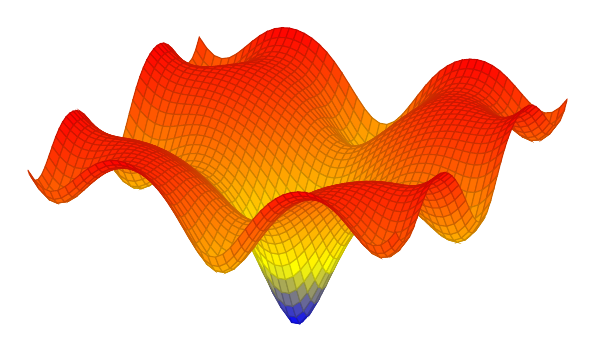
\begin{tikzpicture}
    \begin{axis}[
        xlabel={$x$},
        ylabel={$y$},
        zlabel={$f(x,y)$},
        ticks=none,
        samples=50,
        hide axis           
        ]
        \addplot3[surf, domain=-1.1:1.1, domain y=-1.1:1.1] {
            % Ackley's function
            -20*exp(-0.2*sqrt(0.5*(x^2+y^2))) - exp(0.5*(cos(deg(2*pi*x))+cos(deg(2*pi*y)))) + exp(1) + 20
            };
    \end{axis}
\end{tikzpicture}


As it turns out, neural networks operate in very high dimensional spaces, and there local minima are quite rare, 
it is much more likely that a point where the derivative is $0$ is a saddle point.

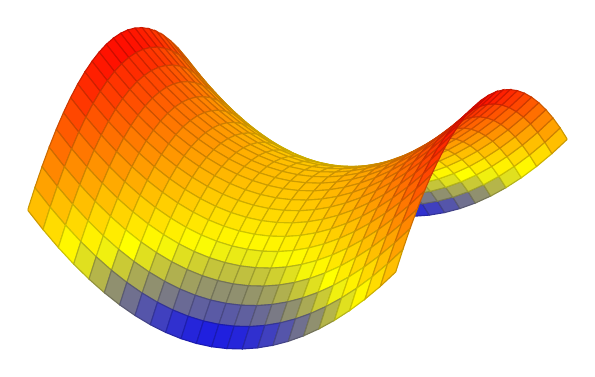
\begin{tikzpicture}
    \begin{axis}[
        xlabel={$x$},
        ylabel={$y$},
        zlabel={$f(x,y)$},
        ticks=none,
        hide axis
    ]
    \addplot3[surf, domain=-2:2, domain y=-2:2] {x^2-y^2};
    \end{axis}
\end{tikzpicture}

The reason for this is that for a point with derivative 0 to be a minimum, the function needs to be concave in all dimensions in that point, which is very unlikely in high dimensional spaces.

A more likely problem to encounter is plateaus, where the algorithm ends up traveling slowly across an almost flat "surface":

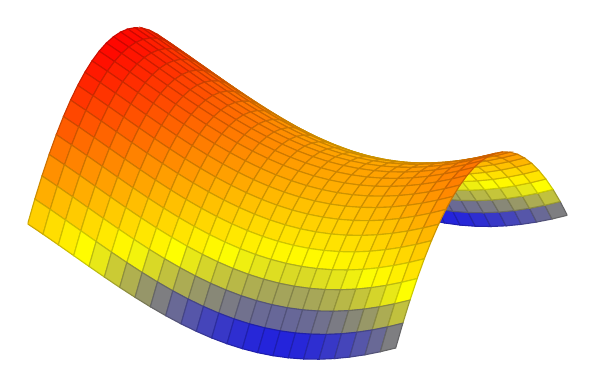
\begin{tikzpicture}
    \begin{axis}[
        xlabel={$x$},
        ylabel={$y$},
        zlabel={$f(x,y)$},
        ticks=none,
        hide axis
    ]
    \addplot3[surf, domain=-4:2, domain y=-2:2] {(x/2)^2 - (x/4)^4 - (1*y)^2};
    \end{axis}
\end{tikzpicture}
